\section{Classification on Fashion MNIST}
\textit{Fashion MNIST}\cite{fashionmnist} is a dataset consisting of a training set of 60,000 examples and a test set of 10,000 examples.
Each example in the dataset is a 28x28 grayscale image belonging to precisely one of 10 classes, presented in Table \ref{table:experiments:classification:fashion-mnist-labels}. 
\begin{table}[H]
    \centering
    \begin{tabularx}{0.8\textwidth} { 
          | >{\centering\arraybackslash}X 
          | >{\centering\arraybackslash}X | }
         \hline
         \textbf{label}& \textbf{description} \\
         \hline
         0 & T-shirt/top \\
         \hline
         1 & trouser  \\
         \hline
         2 & pullover  \\
         \hline
         3 & dress  \\
         \hline
         4 & coat  \\
         \hline
         5 & sandal  \\
         \hline
         6 & shirt  \\
         \hline
         7 & sneaker  \\
         \hline
         8 & bag  \\
         \hline
         9 & ankle boot  \\
         \hline
    \end{tabularx}
    \caption{\textit{Fashion MNIST} labels}
    \label{table:experiments:classification:fashion-mnist-labels}
\end{table}
The task for a machine learning algorithm is to classify a given 28x28 grayscale image into precisely one of 10 categories from Table \ref{table:experiments:classification:fashion-mnist-labels}.
\textit{Fashion MNIST} was invented in 2017 as a replacement for \textit{MNIST}\cite{mnist}. \textit{MNIST}\cite{mnist} has been used as a benchmark for novel and existing algorithms. However, it turns out to be quite easy for modern algorithms and it is not representative of modern computer vision tasks. \textit{Fashion MNIST} is slightly more difficult, but still small enough for experimenting with limited computational resources. This makes it suitable for our purpose.
\begin{figure}[H]
\setlength\extrarowheight{2pt} % for a less-cramped "look"
\centering
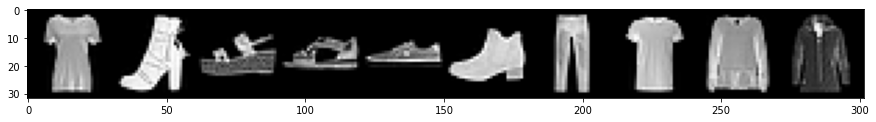
\includegraphics[width=1\textwidth]{experiments/classification/garms-3.png}
\resizebox{\textwidth}{!}{
\begin{tabular}{|c|c|c|c|c|c|c|c|c|c|}
\hline
\text{T-shirt/top}&\text{ankle boot}&\text{sandal}&\text{sandal}&\text{sneaker}&\text{ankle boot}&\text{trousers}&\text{T-shirt/top}&\text{shirt}&\text{coat}\\
\hline
\end{tabular}
}
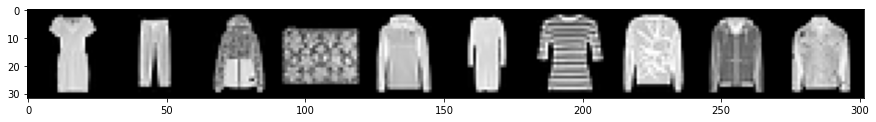
\includegraphics[width=1\textwidth]{experiments/classification/garms-2.png}
\resizebox{\textwidth}{!}{
\begin{tabular}{|c|c|c|c|c|c|c|c|c|c|}
\hline
\text{dress}&\text{trousers}&\text{coat}&\text{bag}&\text{coat}&\text{dress}&\text{T-shirt/top}&\text{pullover}&\text{coat}&\text{coat}\\
\hline
\end{tabular}
}
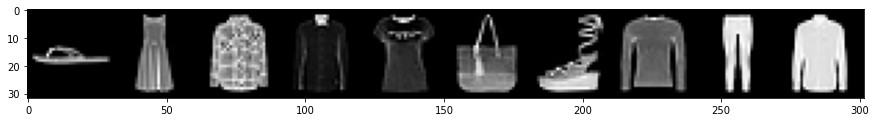
\includegraphics[width=1\textwidth]{experiments/classification/garms-1.png}
\resizebox{\textwidth}{!}{
\begin{tabular}{|c|c|c|c|c|c|c|c|c|c|}
\hline
\text{sandal}&\text{dress}&\text{shirt}&\text{shirt}&\text{T-shirt/top}&\text{bag}&\text{sandal}&\text{pullover}&\text{trousers}&\text{shirt}\\
\hline
\end{tabular}
}
\caption{Some examples from \textit{Fashion MNIST}}
\label{fig.1}
\end{figure}

\subsection{Model}
\label{subsection:experiments:classification:model}
To perform classification experiments, our task is to construct a single neural network that assigns to each given image precisely one of 10 labels from Table \ref{table:experiments:classification:fashion-mnist-labels}. We will begin the discussion by considering theoretical aspects of this problem. We will view each $28 \times 28$ image as a flattened vector in $\R^{784}$.
A way to solve this problem is to interpret it as trying to approximate or learn a 'classification' function which maps an image viewed as a vector  $\R^{784}$ to a vector in $\R^{10}$. In this context, each $i$-th component of an output vector in $\R^{10}$ corresponds to estimated probability that an image belongs to $i$-th class, for $0 \leq i \leq 9$. Hence to assign a label to an image, we assign a label that corresponds to the highest estimated probability. Formally, we want a neural network $\vec{f} : \R^{784} \to \R^{10}$. It turns out that our network can assign labels automatically by using the \textit{softmax} activation function in the output layer. The \textit{softmax} activation function is designed precisely for this use-case. 


From a practical standpoint, we want to have a flexible interface to neural network architecture. This requirement is necessary to support a wide variety of experiments. We want to be able to quickly prototype a new neural network by adding layers or by changing activation function in each layer. Fortunately, PyTorch allows us to achieve both theoretical and practical requirements quite elegantly (see Figure \ref{fig:experiments:classification:model:nn-pytorch}).

\begin{figure}[H]
    \centering
    \begin{minted}[fontsize=\footnotesize]{python}
    from collections import namedtuple
    import torch.nn as nn
    
    image_width = 28
    image_height = 28
    
    LayerConfig = namedtuple("LayerConfig", ["width", "activation"])
    
    class FashionNNMultiHiddens(nn.Module):
    
        def __init__(self, layers_config):
            super(FashionNNMultiHiddens, self).__init__()
    
            previous_width = image_width * image_height
            hidden_layers = []
            for config in layers_config:
                hidden_layers.append(
                    nn.Linear(in_features=previous_width,
                              out_features=config.width))
                hidden_layers.append(config.activation)
                previous_width = config.width
    
            self.nn = nn.Sequential(*hidden_layers)
    
        def forward(self, x):
            return self.nn(x)
    \end{minted}
    \caption{PyTorch implementation of model from Figure \ref{fig:experiments:classification:model:nn} }
    \label{fig:experiments:classification:model:nn-pytorch}
\end{figure}

\begin{figure}[H]
	\centering
	\begin{tikzpicture}[shorten >=1pt]
		\tikzstyle{unit}=[draw,shape=circle,minimum size=1.15cm]
		\tikzstyle{output}=[draw,shape=circle,minimum size=1.15cm,scale=0.9]
		\tikzstyle{hidden}=[draw,shape=circle,fill=black!25,minimum size=1.15cm]
 		\tikzstyle{lasthidden}=[draw,shape=circle,fill=black!25,minimum size=1.15cm,scale=0.8]

		\node[unit](x0) at (0,3.5){$1$};
		\node[unit](x1) at (0,2){$x_1$};
		\node at (0,1){\vdots};
		\node[unit](xd) at (0,0){$x_{784}$};
 
		\node[hidden](h10) at (3,4){$1$};
		\node[hidden](h11) at (3,2.5){$f_{1}^{(1)}$};
		\node at (3,1.5){\vdots};
		\node[hidden](h1m) at (3,-0.5){$f_{n_{(1)}}^{(1)}$};
 
		\node(h22) at (5,0){};
		\node(h21) at (5,2){};
		\node(h20) at (5,4){};
		
		\node(d3) at (6,0){$\ldots$};
		\node(d2) at (6,2){$\ldots$};
		\node(d1) at (6,4){$\ldots$};
 
		\node(hL12) at (7,0){};
		\node(hL11) at (7,2){};
		\node(hL10) at (7,4){};
		
		\node[hidden](hL0) at (9,4){$1$};
		\node[lasthidden](hL1) at (9,2.5){$f_1^{(L-1)}$};
		\node at (9,1.5){\vdots};
		\node[lasthidden](hLm) at (9,-0.5){$f_{n_{(L-1)}}^{(L-1)}$};
 
		\node[output](y1) at (12,3.5){$f_{1}^{(L)}$};
		\node[output](y2) at (12,2){$f_{2}^{(L)}$};
		\node at (12,1){\vdots};	
		\node[output](yc) at (12,0){$f_{10}^{(L)}$};
 
		\draw[->] (x0) -- (h11);
		\draw[->] (x0) -- (h1m);
 
		\draw[->] (x1) -- (h11);
		\draw[->] (x1) -- (h1m);
 
		\draw[->] (xd) -- (h11);
		\draw[->] (xd) -- (h1m);
 
		\draw[->] (hL0) -- (y1);
		\draw[->] (hL0) -- (yc);
		\draw[->] (hL0) -- (y2);
 
		\draw[->] (hL1) -- (y1);
		\draw[->] (hL1) -- (yc);
		\draw[->] (hL1) -- (y2);
 
		\draw[->] (hLm) -- (y1);
		\draw[->] (hLm) -- (y2);
		\draw[->] (hLm) -- (yc);
 
		\draw[->,path fading=east] (h10) -- (h21);
		\draw[->,path fading=east] (h10) -- (h22);
		
		\draw[->,path fading=east] (h11) -- (h21);
		\draw[->,path fading=east] (h11) -- (h22);
		
		\draw[->,path fading=east] (h1m) -- (h21);
		\draw[->,path fading=east] (h1m) -- (h22);
		
		\draw[->,path fading=west] (hL10) -- (hL1);
		\draw[->,path fading=west] (hL11) -- (hL1);
		\draw[->,path fading=west] (hL12) -- (hL1);
		
		\draw[->,path fading=west] (hL10) -- (hLm);
		\draw[->,path fading=west] (hL11) -- (hLm);
		\draw[->,path fading=west] (hL12) -- (hLm);
		
		\draw [decorate,decoration={brace,amplitude=10pt},xshift=-4pt,yshift=0pt] (-0.5,4) -- (0.75,4) node [black,midway,yshift=+0.6cm]{input layer};
		\draw [decorate,decoration={brace,amplitude=10pt},xshift=-4pt,yshift=0pt] (2.5,4.5) -- (3.75,4.5) node [black,midway,yshift=+0.6cm]{$1^{\text{st}}$ hidden layer};
		\draw [decorate,decoration={brace,amplitude=10pt},xshift=-4pt,yshift=0pt] (8.5,4.5) -- (9.75,4.5) node [black,midway,yshift=+0.6cm]{$(L-1)^{\text{th}}$ hidden layer};
		\draw [decorate,decoration={brace,amplitude=10pt},xshift=-4pt,yshift=0pt] (11.5,4) -- (12.75,4) node [black,midway,yshift=+0.6cm]{output layer};
	\end{tikzpicture}
	\caption[Network graph for a \textit{Fashion MNIST} classification.]{This figure illustrates a network graph for a \textit{Fashion MNIST} classification neural network. Output layer is fixed and uses \textit{softmax} activation function. Depending on experiment, other hidden layers vary in width and the activation function. More general implementation of this model is given in Figure \ref{fig:experiments:classification:model:nn-pytorch}.}
	\label{fig:experiments:classification:model:nn}
\end{figure}

\subsection{Methodology}
\label{section:experiments:classification:experiments-methodology}

Each experiment consists of a neural network architecture configuration and a training configuration. Experiments are run independently. 
Each experiment run consists of instantiation of a neural network from the configuration and training from scratch using training configuration from Table \ref{table:expriments:training_config}. In each experiment, the neural network architecture is fixed and only weights and biases are changed by the optimizer. After every 100 batch iterations, training and validation set accuracy and loss are computed for the experiment neural network architecture. The model achieving the best validation accuracy is maintained and its weights are saved. Plots in the subsequent sections were created by manual inspection and analysis of the following statistics:
\begin{itemize}[noitemsep]
    \item training and validation loss collected during the training process,
    \item training and validation accuracy collected during the training process,
    \item validation set accuracy and loss corresponding to the best weights,
    \item class-specific validation set accuracy corresponding to the best weights,
    \item confusion matrix corresponding to the model with the best weights.
\end{itemize}
\begin{figure}[H]
    \centering
    \begin{minted}[fontsize=\footnotesize]{python}
    layer_width = 64
    layers_number = 4
    layers = [ LayerConfig(layer_width, nn.ReLU()) for _ in range(layers_number) ]
    experiment = {
        'name' : 'nn-4x-64-relu-softmax',
        'epochs': 10,
        'batch_size' : 32,
        'layers_config': layers + [LayerConfig(10, nn.Softmax(dim=0))]
    }
    \end{minted}
    \caption{The configuration of \textit{nn-4x-64-relu-softmax} experiment}
    \label{fig:experiments:classification:experiment-example}
\end{figure}

\pagebreak
\subsection{The choice of an optimizer}
\label{subsection:experiments:classification:optimizer}
When it comes to optimizers, in this thesis we only discussed stochastic gradient descent. We briefly mentioned other methods of practical importance. However, the convergence of stochastic gradient descent was too slow under configuration from Table \ref{table:expriments:training_config} (see Table \ref{table:experiments:classification:optimizers-sigmoid} and Table \ref{table:experiments:classification:optimizers-relu}). 
Since the computational resources were limited, after experimenting with different optimizers, Adam produced the best results in the smallest number of training epochs. Adam is currently one of the most popular optimizers and it is a common default choice. The choice of an optimizer is a good example of a practical problem that is not discussed in the approximation theory of neural networks. Theoretical results are completely disconnected from choices regarding the optimization algorithm and its configuration. However, those may significantly affect the performance of the resulting neural network. Effects are especially noticeable when training for a fixed number of epochs, which is a very common practice. Given the fact an average training time of a network with a single hidden layer was about 30 minutes, the training time was indeed significantly affected. This observation was neatly summarised in \citetitle{ruder_2017_an} \cite{ruder_2017_an}, quoted below.

\begin{displayquote}[\citetitle{ruder_2017_an} \cite{ruder_2017_an}, p.10]
"Interestingly, many recent papers use vanilla SGD without momentum and a simple learning rate
annealing schedule. As has been shown, SGD usually achieves to find a minimum, but it might take
significantly longer than with some of the optimizers, is much more reliant on a robust initialization
and annealing schedule, and may get stuck in saddle points rather than local minima. Consequently,
if you care about fast convergence and train a deep or complex neural network, you should choose
one of the adaptive learning rate methods."
\end{displayquote}

The following results were obtained by changing the optimizer in configuration from Table \ref{table:expriments:training_config}. All optimizers were initialized with a default configuration.

\begin{table}[H]
    \centering
    \begin{tabular}{ | c | c | c | }
         \hline
         \textbf{model} & \textbf{SGD} & \textbf{Adam} \\
         \hline
         nn-16-sigmoid-softmax & 70.9800\% & 79.2200\% \\
         \hline
         nn-32-sigmoid-softmax & 70.8300\% & 79.8700\% \\
         \hline
         nn-64-sigmoid-softmax & 70.1500\% & 79.0100\% \\
         \hline
         nn-128-sigmoid-softmax & 68.6500\% & 79.4500\% \\
         \hline
    \end{tabular}

    \caption{validation set accuracy of sigmoid networks after 5 training epochs}
    \label{table:experiments:classification:optimizers-sigmoid}
\end{table}
\begin{table}[H]
    \centering
    \begin{tabular}{ | c | c | c | }
         \hline
         \textbf{model} & \textbf{SGD} & \textbf{Adam} \\
         \hline
         nn-16-relu-softmax & 72.5100\% & 76.7800\% \\
         \hline
         nn-32-relu-softmax & 72.5400\% & 76.6100\% \\
         \hline
         nn-64-relu-softmax & 72.8500\% & 77.2100\% \\
         \hline
         nn-128-relu-softmax & 72.8900\% & 77.4200\% \\
         \hline
    \end{tabular}

    \caption{validation set accuracy of ReLU networks after 5 training epochs}
    \label{table:experiments:classification:optimizers-relu}
\end{table}
\subsection{Impact of batch size on validation accuracy}
\label{subsection:experiments:classification:batch}
Although the batch size seems unimportant in comparison with neural network architecture and the choice of an optimizer, the experimental data from Figure \ref{figure:experiments:classification:batch-size-plot} indicates that the batch size plays an important role when the network is trained for a fixed number of iterations. To examine the effects of various batch sizes, a reasonably large neural network architecture is chosen and such a network is trained using the configuration from Table \ref{table:expriments:training_config}. In this experiment, only the batch size and activation function are varied. It is very important to note that the number of epochs remained unchanged. 

The results displayed in Figure \ref{figure:experiments:classification:batch-size-plot} indicate that training using smaller batch sizes results in significantly greater validation accuracy. This can be attributed to the fact that a smaller batch size implies a greater number of parameter updates since the number of epochs is fixed. It is worth noting that such a training setup requires significantly more time. For instance, the average training time using a batch size of 32 examples was about 30 minutes, while the average training time using the batch size of 256 examples was about 5 minutes. The accuracy drop after the batch size of 128 is noticeable for every activation function. This could be expected since the number of parameter updates drops significantly. On the other hand, a larger batch size often results in a more accurate estimate of the gradient.

It seems that larger batch sizes generally require a larger number of training epochs, which is indeed sensible, as the optimization performs significantly less parameter updates. It is reasonable to conjecture that the sweet spot for the default training configuration is a batch size of 64 examples, as it seems that such a configuration performs slightly better than other batch sizes in 2 out of 3 activation functions.

To sum up, batch size likely plays an important role in training a neural network. The results discussed are relevant only for one neural network architecture and one default training setup. However, according to the Figure 1 from \cite{hoffer_2018_train} and Figure 2 from \cite{shirishkeskar_2017_on}, the similar observations can be made on more complex datasets and neural networks. It is interesting to note that \cite{hoffer_2018_train} and \cite{shirishkeskar_2017_on} provide different explanations and analysis of this phenomenon.

\begin{figure}[H]
    \centering
    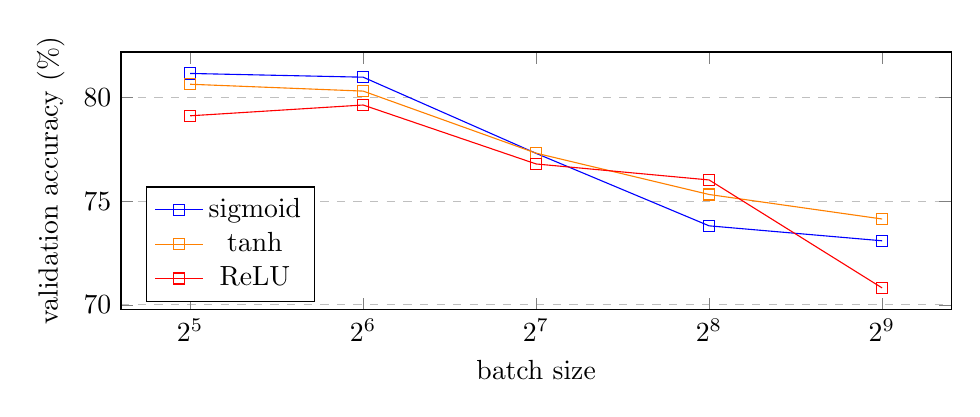
\begin{tikzpicture}
        \begin{axis}[
            height=0.4\textwidth,
            width=\textwidth,
            xlabel={batch size},
            ylabel={validation accuracy (\%)},
            ymajorgrids=true,
            grid style=dashed,
            xmode=log,
            legend pos=south west,
            log basis x={2}]
            \addplot[mark=square,blue] coordinates {(32,81.15) (64,80.97) (128,77.30) (256,73.81) (512,73.09)};
            \addplot[mark=square,orange] coordinates {(32,80.63) (64,80.30) (128,77.31) (256,75.32) (512,74.14)};
            \addplot[mark=square,red] coordinates {(32,79.11) (64,79.63) (128,76.79) (256,76.02) (512,70.82)};
            \legend{sigmoid, tanh, ReLU}
        \end{axis}
    \end{tikzpicture}
    \caption{Effects of various batch sizes on training \textit{nn-2x-128-sigmoid-softmax}}
    \label{figure:experiments:classification:batch-size-plot}
\end{figure}
\subsection{Impact of activation function on validation accuracy}
\label{subsection:experiments:classification:activation}
Since the activation function gives rise to nonlinearity, it is reasonable to conjecture that the activation function affects performance. In \nameref{chapter:literature-review} and \nameref{chapter:universality}, we have also observed that the properties of activation function also play an essential role in many proofs of universality.

To begin an experimental study of the effects of the activation function, we will focus on neural networks with a single hidden layer. Each neural network is trained using the configuration from Table \ref{table:expriments:training_config}. In this experiment, only the hidden layer width and the activation function are varied. For each experiment configuration, the model achieving the best validation accuracy is saved and used in the following analysis.

According to the results displayed in Figure \ref{fig:experiments:classification:all-activations-plot}, it is likely that the activation function significantly affects validation set accuracy, given current training configuration. Thus, it is reasonable to conjecture that the activation function affects the generalization error. It is interesting to note that sigmoid and $\tanh$ significantly and consistently outperform $\operatorname{ReLU}$ regardless of hidden layer width. That is slightly surprising because many modern neural network architectures use $\operatorname{ReLU}$ and similar rectified activation functions instead of $\operatorname{sigmoid}$ and $\tanh$.

It can be shown that $\operatorname{sigmoid}$  and $\tanh$ are algebraically related. More precisely, for every $x \in \R, \tanh{(x)} = 2\sigma(2x) - 1$. Given the structure of a fully-connected neural network and this algebraic connection, it is reasonable to expect that $\operatorname{sigmoid}$  and $\tanh$ produce similar results. According to the results displayed in Figure \ref{fig:experiments:classification:all-activations-plot}, that is indeed the case. Another surprising observation is the significant validation accuracy drop for $\operatorname{ReLU}$ networks after hidden layer width of 128 neurons. Although ReLU networks perform worse as the hidden layer width increases, it seems that $\operatorname{sigmoid}$ and $\tanh$ networks perform better. The widest $\tanh$ and $\operatorname{sigmoid}$ achieve the best validation accuracy. We will briefly discuss the worst $\operatorname{ReLU}$ model. According to the Figure \ref{fig:experiments:classification:wide-relu-plot}, validation and test accuracy are consistently very similar. Hence, there is no evidence of overfitting.

\begin{figure}[H]
    \begin{minipage}{.5\textwidth}
        \centering
        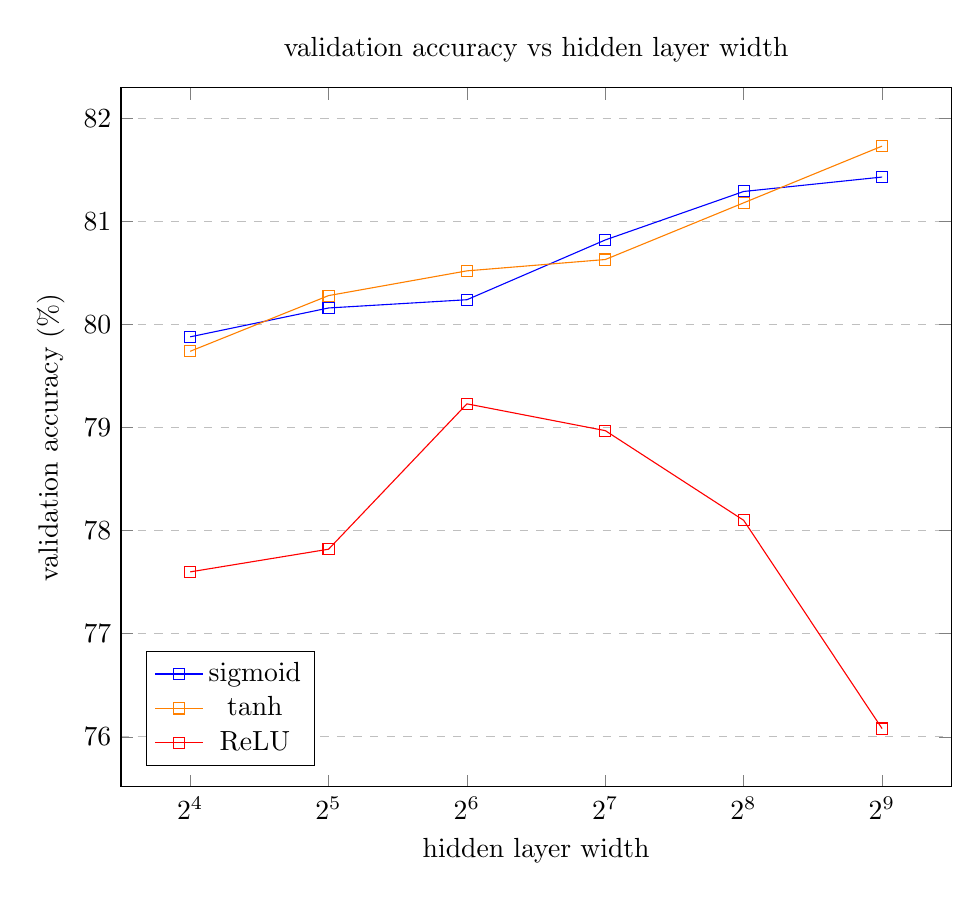
\begin{tikzpicture}
            \begin{axis}[
                width=\textwidth,
                title={validation accuracy vs hidden layer width},
                xlabel={hidden layer width},
                ylabel={validation accuracy (\%)},
                ymajorgrids=true,
                grid style=dashed,
                xmode=log,
                legend pos=south west,
                log basis x={2}]
                \addplot[mark=square,blue] coordinates {(16,79.88) (32,80.16) (64,80.24) (128,80.82) (256,81.29) (512,81.43)};
                \addplot[mark=square,orange] coordinates {(16,79.74) (32,80.28) (64,80.52) (128,80.63) (256,81.18) (512,81.73)};
                \addplot[mark=square,red] coordinates {(16,77.60) (32,77.82) (64,79.23) (128,78.97) (256,78.10) (512,76.08)};
                \legend{sigmoid, tanh, ReLU}
            \end{axis}
        \end{tikzpicture}
        \captionof{figure}{Validation accuracy of the best model with given hidden layer width and activation function}
        \label{fig:experiments:classification:all-activations-plot}
    \end{minipage}%
    \hspace{0.5cm}
    \begin{minipage}{.5\textwidth}
        \centering
        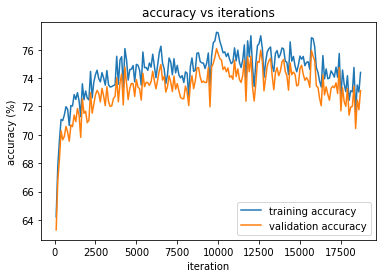
\includegraphics[scale=0.5]{experiments/classification/relu-single-layer-no-overfitting.png}
        \captionof{figure}{Training and validation accuracy of $\operatorname{ReLU}$ network with a single hidden layer of 512 neurons. This is the worst $\operatorname{ReLU}$ model in this experiment.}
        \label{fig:experiments:classification:wide-relu-plot}
    \end{minipage}
\end{figure}


\subsection{Adding a layer}
\label{subsection:experiments:classification:adding-a-layer}
In this subsection, we will focus on neural networks with two hidden layers of the same width. The experiment configuration is almost identical to one from the previous section. The only change is the addition of another identical hidden layer to each neural network.
For each experiment configuration, the model achieving the best validation accuracy is saved and used in the following analysis.

From Figure \ref{fig:experiments:classification:all-activations-plot}, it is noticeable that the best validation accuracy increases consistently with the hidden layer width. This may suggest that $\operatorname{sigmoid}$ and $\operatorname{tanh}$ neural networks may benefit from the increased model complexity. However, it seems that this does not happen to the extent one may expect (see Figure \ref{fig:experiments:classification:adding-a-layer-all-activations}).

In the previous section, we discussed the similarity between the $\operatorname{sigmoid}$ and $\operatorname{tanh}$ activation function. From the Figure \ref{fig:experiments:classification:adding-a-layer-all-activations}, we can conclude that $\operatorname{sigmoid}$ and $\operatorname{tanh}$ networks remain achieving similar validation accuracy, what is compatible with results from the previous section.

From Figure \ref{fig:experiments:classification:adding-a-layer-sigmoid}, Figure \ref{fig:experiments:classification:adding-a-layer-tanh} and Figure \ref{fig:experiments:classification:adding-a-layer-relu}, it is evident that the layer addition results in slightly better validation accuracy for layer widths up to and including 128 neurons. However, the difference is mostly within $1.5\%$ and this can be attributed to the noise. It is hard to say whether the validation accuracy boost is significant. According to the benchmark table in \cite{fashionmnistgithub}, similar neural networks may achieve the validation accuracy of $88\%$ (see the entry for \textit{MLP 256-128-100}). The pattern is slightly unclear for layer widths larger than 128 neurons. For instance, the network with $\operatorname{tanh}$ activation and two hidden layers of 512 neurons achieved the validation accuracy of $82.33\%$, which is the best validation accuracy so far. However, such a configuration performed noticeably less well for other activation functions, especially $\operatorname{ReLU}$.

Neural networks with $\operatorname{tanh}$ activation function benefited the most from the extra layer. According to Figure \ref{fig:experiments:classification:adding-a-layer-tanh}, $\operatorname{tanh}$ neural networks with two identical layers consistently performed at least as well as the corresponding single layer configuration. It is interesting to note that $\operatorname{ReLU}$ networks benefited the least from the extra layer. This observation is quite evident from the Figure \ref{fig:experiments:classification:adding-a-layer-relu}. As in the case of neural networks with the single layer, $\operatorname{ReLU}$ networks seem to generalize slightly worse than $\operatorname{tanh}$ and $\operatorname{sigmoid}$ networks.

\begin{figure}[H]
    \centering
    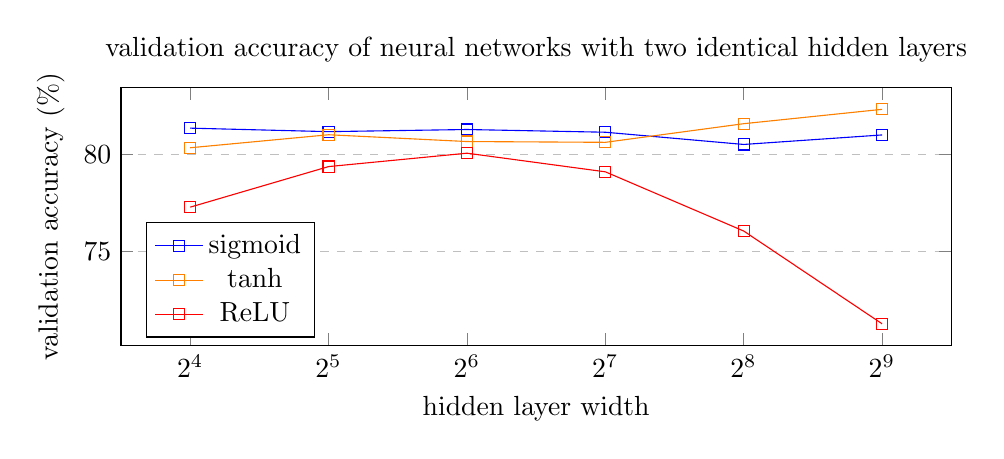
\begin{tikzpicture}
        \begin{axis}[
            height=0.4\textwidth,
            title={validation accuracy of neural networks with two identical hidden layers},
            width=\textwidth,
            xlabel={hidden layer width},
            ylabel={validation accuracy (\%)},
            ymajorgrids=true,
            grid style=dashed,
            xmode=log,
            legend pos=south west,
            log basis x={2}]
            \addplot[mark=square,blue] coordinates {(16,81.36) (32,81.18) (64, 81.29) (128,81.15) (256,80.52) (512,81.01)};
            \addplot[mark=square,orange] coordinates {(16,80.35) (32,81.02) (64,80.67) (128,80.63) (256,81.59) (512,82.33)};
            \addplot[mark=square,red] coordinates {(16,77.29) (32,79.38) (64,80.07) (128,79.11) (256,76.06) (512,71.28)};
            \legend{sigmoid, tanh, ReLU}
        \end{axis}
    \end{tikzpicture}
    \caption{Validation accuracy for networks with two identical hidden layers}
    \label{fig:experiments:classification:adding-a-layer-all-activations}
\end{figure}
\newpage
\begin{figure}[H]
    \centering
    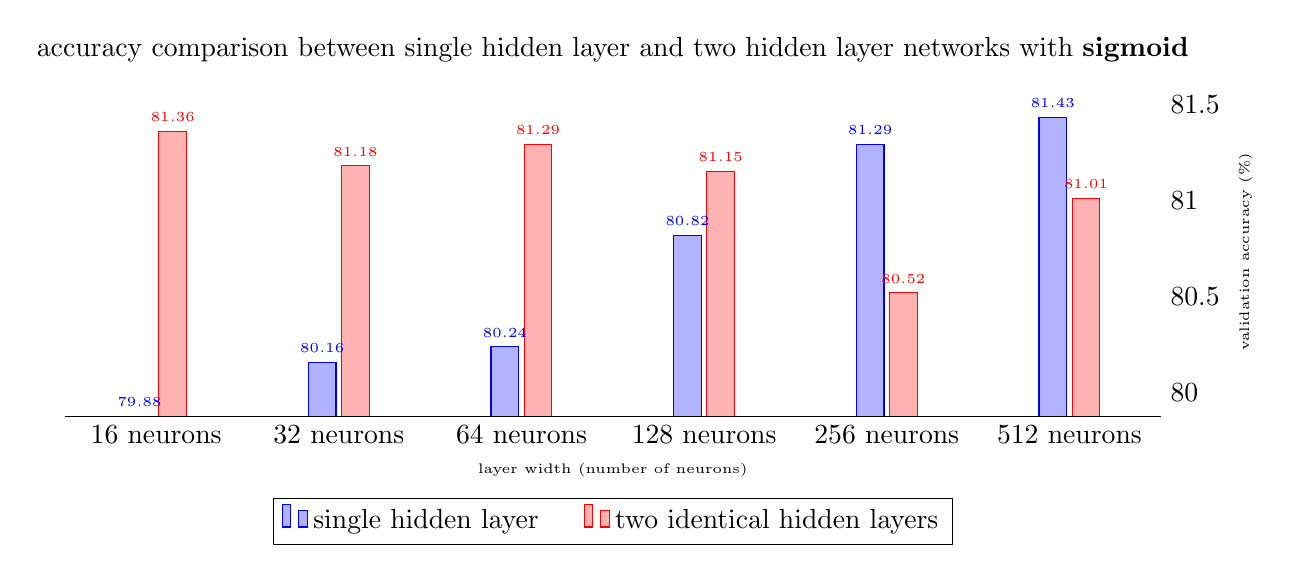
\begin{tikzpicture}
      \centering
      \begin{axis}[
            ybar, axis on top,
            title={accuracy comparison between single hidden layer and two hidden layer networks with \textbf{sigmoid}},
            height=5.75cm, width=15.5cm,
            tick align=inside,
            enlarge y limits={value=.1,upper},
            axis x line*=bottom,
            axis y line*=right,
            y axis line style={opacity=0},
            tickwidth=0pt,
            enlarge x limits=true,
            legend style={
                at={(0.5,-0.25)},
                anchor=north,
                legend columns=-1,
                /tikz/every even column/.append style={column sep=0.5cm}
           },
           ylabel={validation accuracy (\%)},
           symbolic x coords={
               16 neurons, 32 neurons, 64 neurons, 128 neurons,
               256 neurons, 512 neurons
           },
           xtick=data,
           xlabel={layer width (number of neurons)},
           label style={font=\tiny},
           every node near coord/.append style={font=\tiny},
           nodes near coords={
            \pgfmathprintnumber[precision=2]{\pgfplotspointmeta}
           }
        ]
        \addplot coordinates {
            (16 neurons,79.88) 
            (32 neurons,80.16) 
            (64 neurons,80.24) 
            (128 neurons,80.82) 
            (256 neurons,81.29) 
            (512 neurons,81.43)
        };
        \addplot coordinates {
            (16 neurons,81.36) 
            (32 neurons,81.18) 
            (64 neurons, 81.29) 
            (128 neurons,81.15) 
            (256 neurons,80.52) 
            (512 neurons,81.01)
        };
        \legend{single hidden layer, two identical hidden layers}
      \end{axis}
    \end{tikzpicture}
    \caption{Validation accuracy for \textbf{sigmoid}  grouped by number of layers}
    \label{fig:experiments:classification:adding-a-layer-sigmoid}
\end{figure}
\begin{figure}[H]
    \centering
    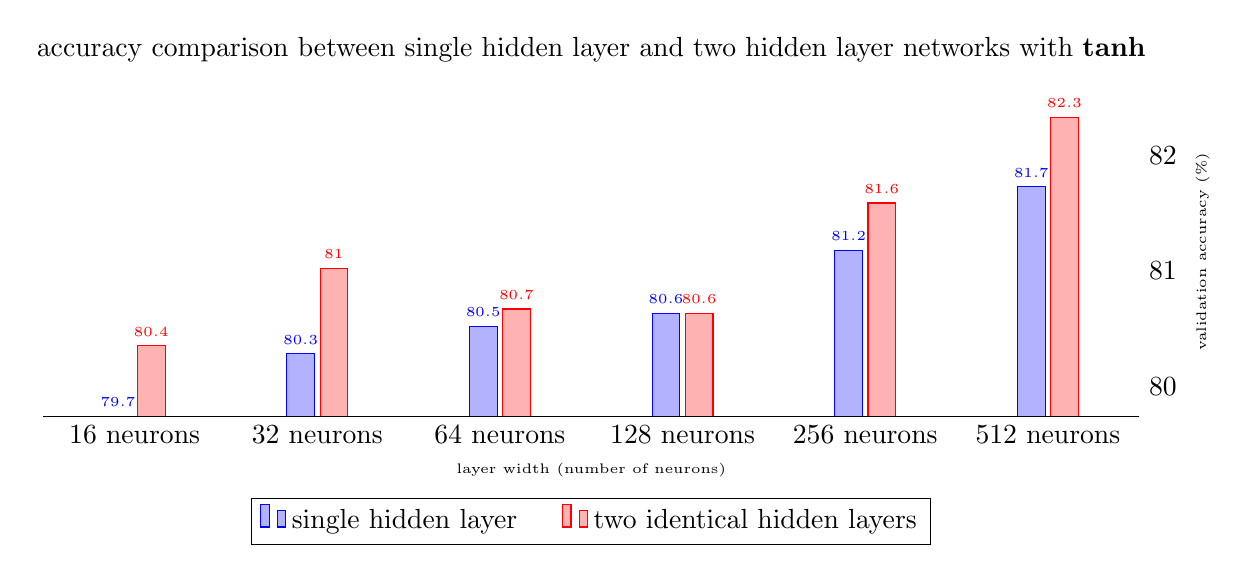
\begin{tikzpicture}
      \centering
      \begin{axis}[
            ybar, axis on top,
            title={accuracy comparison between single hidden layer and two hidden layer networks with \textbf{tanh}},
            height=5.75cm, width=15.5cm,
            tick align=inside,
            enlarge y limits={value=.1,upper},
            axis x line*=bottom,
            axis y line*=right,
            y axis line style={opacity=0},
            tickwidth=0pt,
            enlarge x limits=true,
            legend style={
                at={(0.5,-0.25)},
                anchor=north,
                legend columns=-1,
                /tikz/every even column/.append style={column sep=0.5cm}
           },
           ylabel={validation accuracy (\%)},
            symbolic x coords={
               16 neurons, 32 neurons, 64 neurons, 128 neurons,
               256 neurons, 512 neurons
            },
           xtick=data,
           xlabel={layer width (number of neurons)},
           label style={font=\tiny},
           every node near coord/.append style={font=\tiny},
           nodes near coords={
            \pgfmathprintnumber[precision=1]{\pgfplotspointmeta}
           }
        ]
        
        \addplot coordinates {
            (16 neurons,79.74) 
            (32 neurons,80.28) 
            (64 neurons,80.52) 
            (128 neurons,80.63) 
            (256 neurons,81.18) 
            (512 neurons,81.73)
        };
        \addplot coordinates {
            (16 neurons,80.35) 
            (32 neurons,81.02) 
            (64 neurons,80.67) 
            (128 neurons,80.63) 
            (256 neurons,81.59) 
            (512 neurons,82.33)
        };
        \legend{single hidden layer, two identical hidden layers}
      \end{axis}
    \end{tikzpicture}  
    \caption{Validation accuracy for \textbf{tanh} grouped by the number of layers}
    \label{fig:experiments:classification:adding-a-layer-tanh}
\end{figure}
\begin{figure}[H]
    \centering
    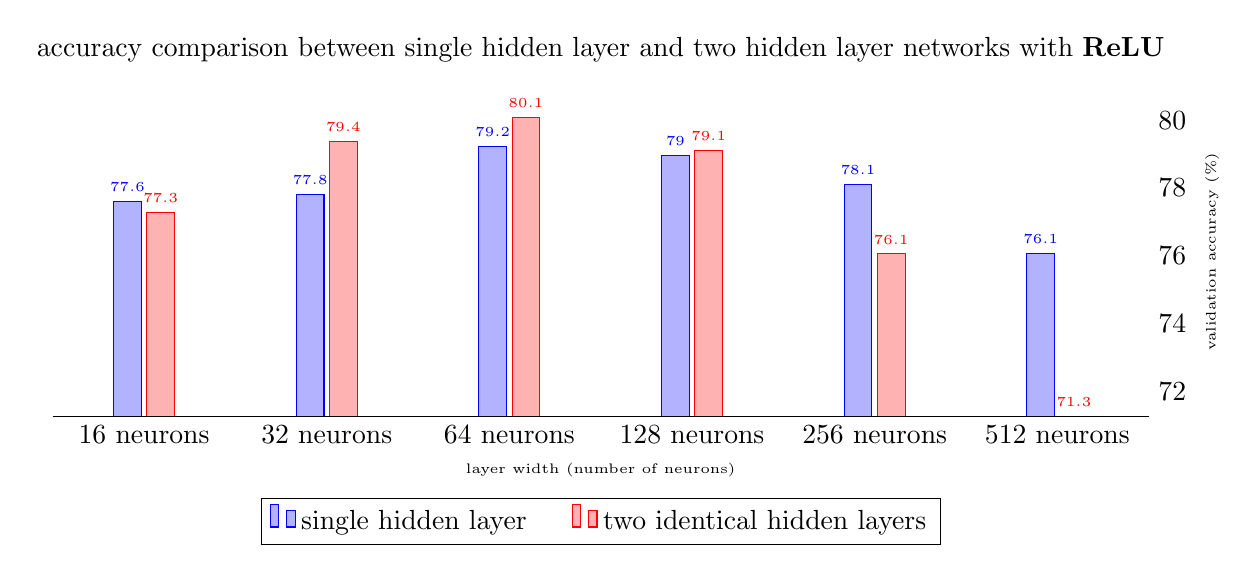
\begin{tikzpicture}
      \centering
      \begin{axis}[
            ybar, axis on top,
            title={accuracy comparison between single hidden layer and two hidden layer networks with \textbf{ReLU}},
            height=5.75cm, width=15.5cm,
            tick align=inside,
            enlarge y limits={value=.1,upper},
            axis x line*=bottom,
            axis y line*=right,
            y axis line style={opacity=0},
            tickwidth=0pt,
            enlarge x limits=true,
            legend style={
                at={(0.5,-0.25)},
                anchor=north,
                legend columns=-1,
                /tikz/every even column/.append style={column sep=0.5cm}
           },
           ylabel={validation accuracy (\%)},
            symbolic x coords={
               16 neurons, 32 neurons, 64 neurons, 128 neurons,
               256 neurons, 512 neurons
            },
           xtick=data,
           label style={font=\tiny},
           xlabel={layer width (number of neurons)},
           every node near coord/.append style={font=\tiny},
           nodes near coords={
            \pgfmathprintnumber[precision=1]{\pgfplotspointmeta}
           }
        ]
        \addplot coordinates {
            (16 neurons,77.60)
            (32 neurons,77.82) 
            (64 neurons,79.23) 
            (128 neurons,78.97) 
            (256 neurons,78.10) 
            (512 neurons,76.08)
        };
        \addplot coordinates {
            (16 neurons,77.29) 
            (32 neurons,79.38) 
            (64 neurons,80.07) 
            (128 neurons,79.11) 
            (256 neurons,76.06) 
            (512 neurons,71.28)
        };
        \legend{single hidden layer, two identical hidden layers}
      \end{axis}
    \end{tikzpicture}  
    \caption{Validation accuracy for \textbf{ReLU} grouped by the number of layers}
    \label{fig:experiments:classification:adding-a-layer-relu}
\end{figure}
\subsection{Impact of neural network depth on validation accuracy}
\label{subsection:experiments:classification:depth}
In this subsection, we will discuss the relationship between the best validation accuracy and neural network depth. The experiment setup and methodology are almost identical to the previous subsection. The only change is the addition of multiple identical hidden layers instead of a single hidden layer.
In the previous subsection, we observed that the addition of a single identical layer did not significantly improve the validation accuracy. According to the results presented in Figure \ref{figure:experiments:classification:depth:64} and in Figure \ref{figure:experiments:classification:depth:128}, validation accuracy does not improve with addition of identically wide hidden layers. Hence, we may conjecture that on this dataset, deeper fully-connected networks do not generalize better than shallow fully-connected networks. It is important to note that results are consistent across all activation functions. 
Moreover, results in Figure \ref{figure:experiments:classification:depth:64} and Figure \ref{figure:experiments:classification:depth:128} are almost identical. This can be attributed to the apparent similarity in neural network architecture.

It is interesting to note that the validation accuracy remains close to $80 \%$ for networks with at most 4 layers. However, as the number of layers increases, the validation accuracy significantly decreases. This observation applies to all activation functions. However the validation accuracy drop is the largest for $\operatorname{sigmoid}$ and $\tanh$. This can be attributed to a well-known \textit{vanishing gradient} problem. We will briefly discuss that source of difficulty in training deep neural networks with $\operatorname{sigmoid}$ activation. We know that $\lim_{x \to \infty} \sigma (x) = 1$ and $\lim_{x \to -\infty} \sigma (x) = 0$. By Lemma \ref{lemma:introduction:activation:sigmoid-derivative}, we conclude that $\lim_{x \to \infty} \sigma'(x) = 0$ and $\lim_{x \to -\infty} \sigma'(x) = 0$. Informally, as the inputs of a $\operatorname{sigmoid}$ layer become extremely small or extremely large, the gradient of the loss function with respect to parameters of a $\operatorname{sigmoid}$ layer vanishes. This causes serious problems in gradient-based optimization since the corresponding weights and biases cease to update. However, in case of $\operatorname{ReLU}$, the drop in validation accuracy resulting from increased depth is noticeably smaller than in case of $\operatorname{sigmoid}$ and $\tanh$. This is also a known result and one of key reasons why $\operatorname{ReLU}$ is preferred to $\operatorname{sigmoid}$ and $\tanh$ when training deep networks.

\begin{figure}[H]
    \centering
    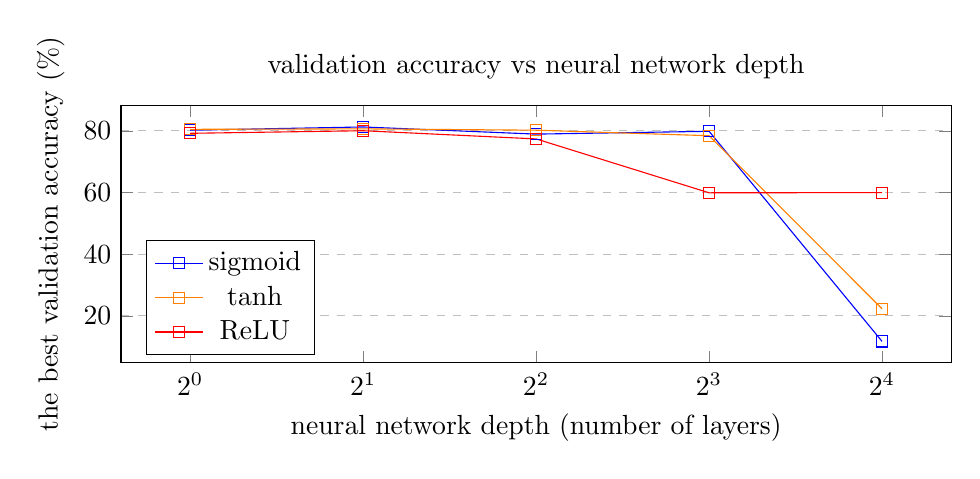
\begin{tikzpicture}
        \begin{axis}[
            height=0.4\textwidth,
            width=\textwidth,
            title= {validation accuracy vs neural network depth},
            xlabel={neural network depth (number of layers)},
            ylabel={the best validation accuracy (\%)},
            ymajorgrids=true,
            grid style=dashed,
            xmode=log,
            legend pos=south west,
            log basis x={2}]
            \addplot[mark=square,blue] coordinates {(1,80.24) (2,81.29) (4, 78.97) (8,79.88) (16,11.72)};
            \addplot[mark=square,orange] coordinates {(1,80.52) (2,80.67) (4,80.24) (8,78.45) (16,22.30)};
            \addplot[mark=square,red] coordinates {(1,79.23) (2,80.07) (4,77.41) (8,59.93) (16,60.00)};
            \legend{sigmoid, tanh, ReLU}
        \end{axis}
    \end{tikzpicture}
    \caption{Effects of varying neural network depth while keeping layer width of \textbf{64 neurons}}
    \label{figure:experiments:classification:depth:64}
\end{figure}
\begin{figure}[H]
    \centering
    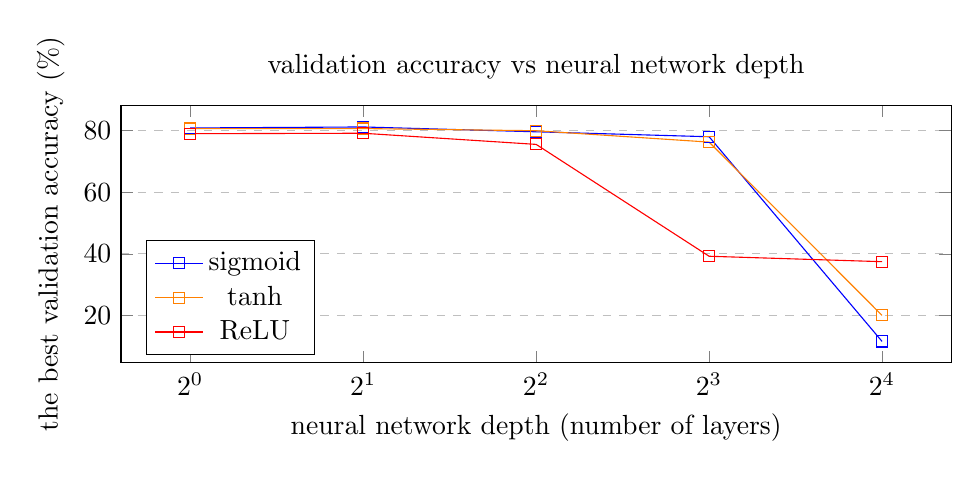
\begin{tikzpicture}
        \begin{axis}[
            height=0.4\textwidth,
            width=\textwidth,
            title= {validation accuracy vs neural network depth},
            xlabel={neural network depth (number of layers)},
            ylabel={the best validation accuracy  (\%)},
            ymajorgrids=true,
            grid style=dashed,
            xmode=log,
            legend pos=south west,
            log basis x={2}]
            \addplot[mark=square,blue] coordinates {(1,80.82) (2,81.15) (4, 79.58) (8,77.98) (16,11.60)};
            \addplot[mark=square,orange] coordinates {(1,80.63) (2,80.63) (4,79.93) (8,76.24) (16,20.05)};
            \addplot[mark=square,red] coordinates {(1,78.97) (2,79.11) (4,75.50) (8,39.22) (16,37.46)};
            \legend{sigmoid, tanh, ReLU}
        \end{axis}
    \end{tikzpicture}
    \caption{Effects of varying neural network depth while keeping layer width of \textbf{128 neurons}}
    \label{figure:experiments:classification:depth:128}
\end{figure}
\subsection{Interesting observation}

According to Figure \ref{figure:experiments:classification:accuracy-per-class-best}, two  models achieving the best validation accuracy, \textit{nn-2x-512-tanh-softmax} and \textit{nn-512-sigmoid-softmax}, demonstrate similar performance on every label.
However, it is interesting to observe that both models struggle with \textit{shirt}s. Although both models perform decently on \textit{pullover} and \textit{T-shirt}, they both perform significantly worse on \textit{shirt}. 

Figure \ref{fig:experiments:classification:best-tanh} demonstrates that the training and accuracy gap of \textit{nn-2x-512-tanh-softmax} remains quite small. However, in Figure \ref{fig:experiments:classification:best-sigmoid}, we can observe slightly larger gap between training and validation accuracy of \textit{nn-512-sigmoid-softmax}. Since the training accuracy of both models peaks at about $82 \%$, there is evidence to suggest both models struggle to fit the training set. Hence, there is no evidence that those networks overfit. In the previous section, we observed that the addition of more fully-connected layers does not significantly affect the generalization. This may indicate that fully-connected architecture is generally too simple for this dataset.


\begin{figure}[H]
    \centering
    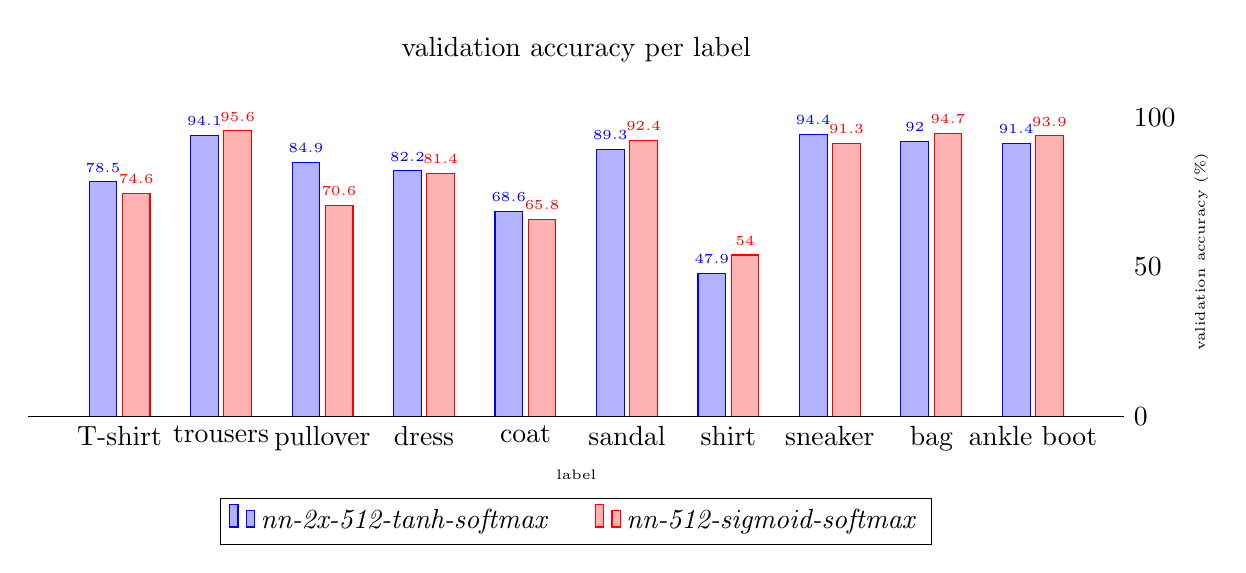
\begin{tikzpicture}
        \begin{axis}[
            symbolic x coords={T-shirt,trousers,pullover,dress,coat,sandal,shirt,sneaker,bag,ankle boot},
            width=15.5cm,
            height=5.75cm,
            ymax=100,
            ymin=0,
            xtick=data,
            ybar, axis on top,
            title={validation accuracy per label},
            height=5.75cm, width=15.5cm,
            tick align=inside,
            enlarge y limits={value=.1,upper},
            axis x line*=bottom,
            axis y line*=right,
            y axis line style={opacity=0},
            tickwidth=0pt,
            enlarge x limits=true,
            legend style={
                at={(0.5,-0.25)},
                anchor=north,
                legend columns=-1,
                /tikz/every even column/.append style={column sep=0.5cm}
           },
           ylabel={validation accuracy (\%)},
           xtick=data,
           xlabel={label},
           label style={font=\tiny},
           every node near coord/.append style={font=\tiny},
           nodes near coords={
            \pgfmathprintnumber[precision=2]{\pgfplotspointmeta}
           }
        ]
            \addplot coordinates {
                (T-shirt, 78.50)
                (trousers, 94.10)
                (pullover, 84.90)
                (dress, 82.20)
                (coat, 68.60)
                (sandal, 89.30)
                (shirt, 47.90)
                (sneaker, 94.40)
                (bag, 92.00)
                (ankle boot, 91.40)
            };
            \addplot coordinates {
                (T-shirt, 74.60)
                (trousers, 95.60)
                (pullover, 70.60)
                (dress, 81.40)
                (coat, 65.80)
                (sandal, 92.40)
                (shirt, 54.00)
                (sneaker, 91.30)
                (bag, 94.70)
                (ankle boot, 93.90)
            };
            \legend{\textit{nn-2x-512-tanh-softmax},\textit{nn-512-sigmoid-softmax}}
        \end{axis}

    \end{tikzpicture}
    \caption{Validation accuracy per label for the best network configurations}
    \label{figure:experiments:classification:accuracy-per-class-best}
\end{figure}
\begin{figure}[H]
    \begin{minipage}{.5\textwidth}
        \centering
        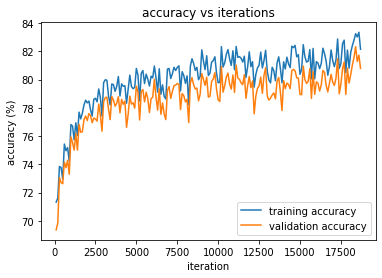
\includegraphics[scale=0.5]{experiments/classification/tanh.png}
        \captionof{figure}{Accuracy pattern of \textit{nn-2x-512-tanh-softmax} }
        \label{fig:experiments:classification:best-tanh}
    \end{minipage}%
    \hspace{0.25cm}
    \begin{minipage}{.5\textwidth}
        \centering
        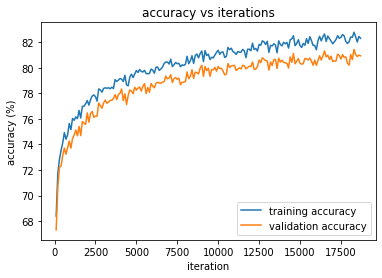
\includegraphics[scale=0.5]{experiments/classification/sigmoid.png}
        \captionof{figure}{Accuracy pattern of \textit{nn-512-sigmoid-softmax}}
        \label{fig:experiments:classification:best-sigmoid}
    \end{minipage}
\end{figure}

\subsection{Conclusion}

In this chapter, we discussed various practical problems related to the applications of neural networks. Despite impressive theoretical properties discussed in \nameref{chapter:literature-review} and \nameref{chapter:universality}, many practical applications of neural networks often suffer from issues not addressed in the universal approximation theory. 

According to state of the art results from  \nameref{chapter:literature-review}, $\operatorname{ReLU}$, $\operatorname{sigmoid}$ and $\operatorname{tanh}$ have comparable theoretical properties. However, in \nameref{subsection:experiments:classification:activation}, we observed that those activation functions result in noticeably different validation accuracy. This can be attributed to the little emphasis we put on the training configuration. This suggests that different activation functions may demand different training configurations. To address a mysterious performance gap between $\operatorname{ReLU}$ and alternatives,
more research is necessary. For example, studying the effects of weight regularisation (weight decay) or employing a more flexible learning rate scheduler could provide more insight into this observation. According to the results reported on the  \href{http://fashion-mnist.s3-website.eu-central-1.amazonaws.com/}{Fashion MNIST benchmark dashboard}, a neural network with a single layer of 100 neurons and $\operatorname{ReLU}$ activation function achieved the accuracy of $87.7\%$. Moreover, such a network outperformed $\tanh$ counterparts. This may suggest that $\operatorname{ReLU}$ networks perform better than observed in this thesis.

We have also observed that the best validation accuracy peaks at about $82\%$.  According to the benchmark table in \cite{fashionmnistgithub}, more sophisticated convolutional neural networks achieve the validation accuracy exceeding $90\%$. This may indicate that the fully-connected architecture is generally too simple to perform the classification on this dataset.

Seemingly unimportant hyperparameter choices discussed in \nameref{subsection:experiments:classification:batch} and \nameref{subsection:experiments:classification:optimizer} are disconnected from the approximation theory of neural networks. However, we observed they may have significant practical consequences.